% !TEX root = BA-Bauer.tex

\newpage
\appendix
\section{Flussdiagramme}
\subsection{Aufnahmefunktion}
\label{fluss:recf}
\begin{figure}[h]
	\begin{center}
		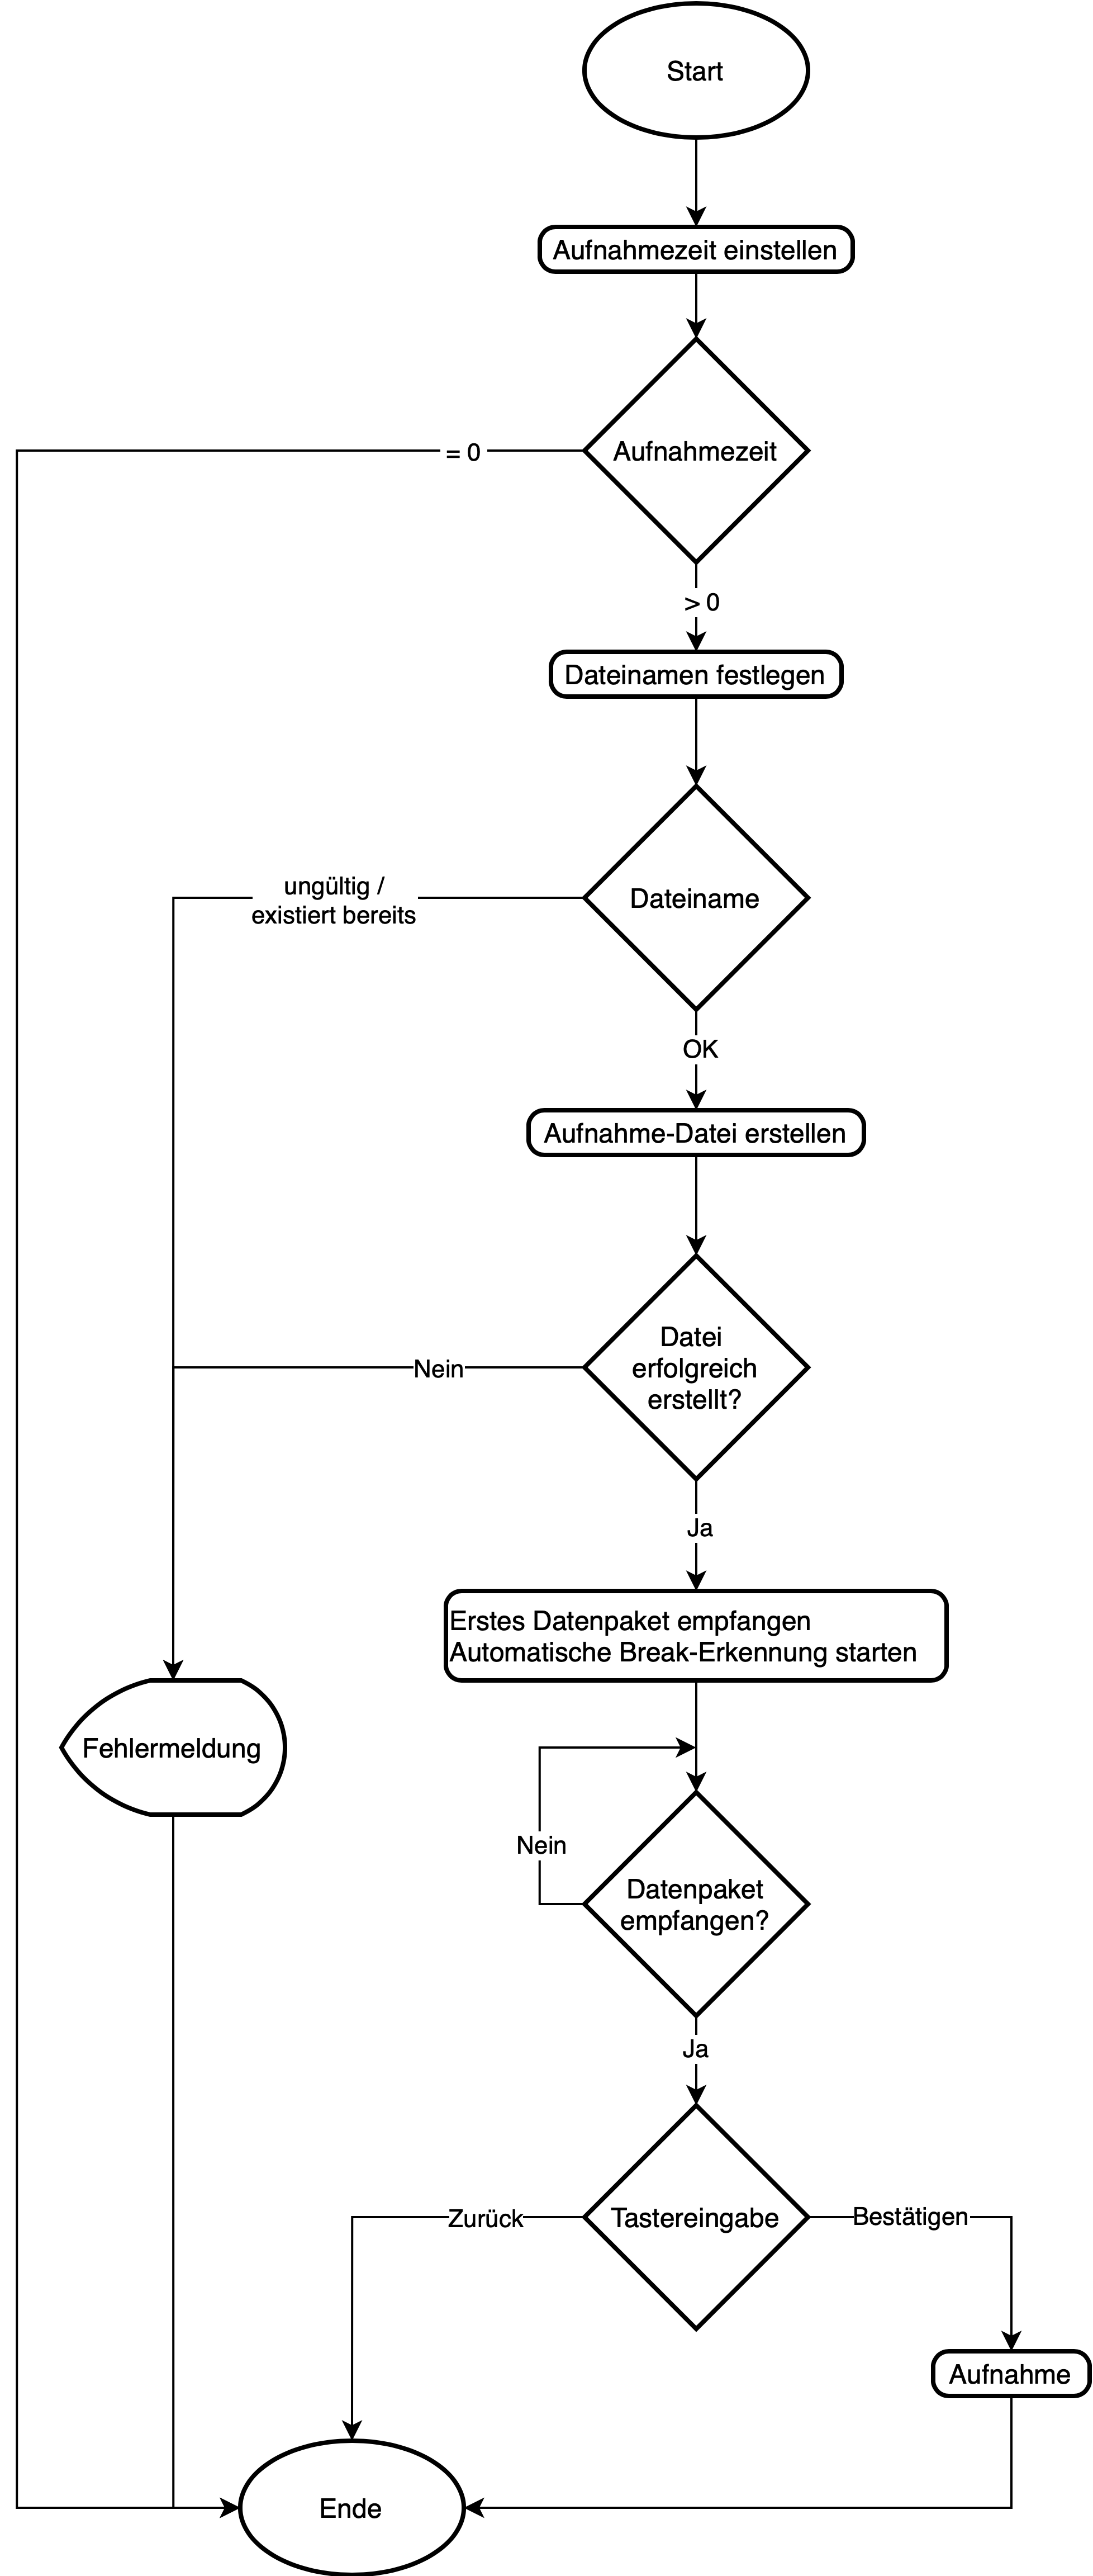
\includegraphics[height=.76\textheight]{Aufnahmefunktion}
	\end{center}
\end{figure}
\newpage
\subsection{Wiedergabefunktion}
\label{fluss:playf}
\begin{figure}[h]
	\begin{center}
		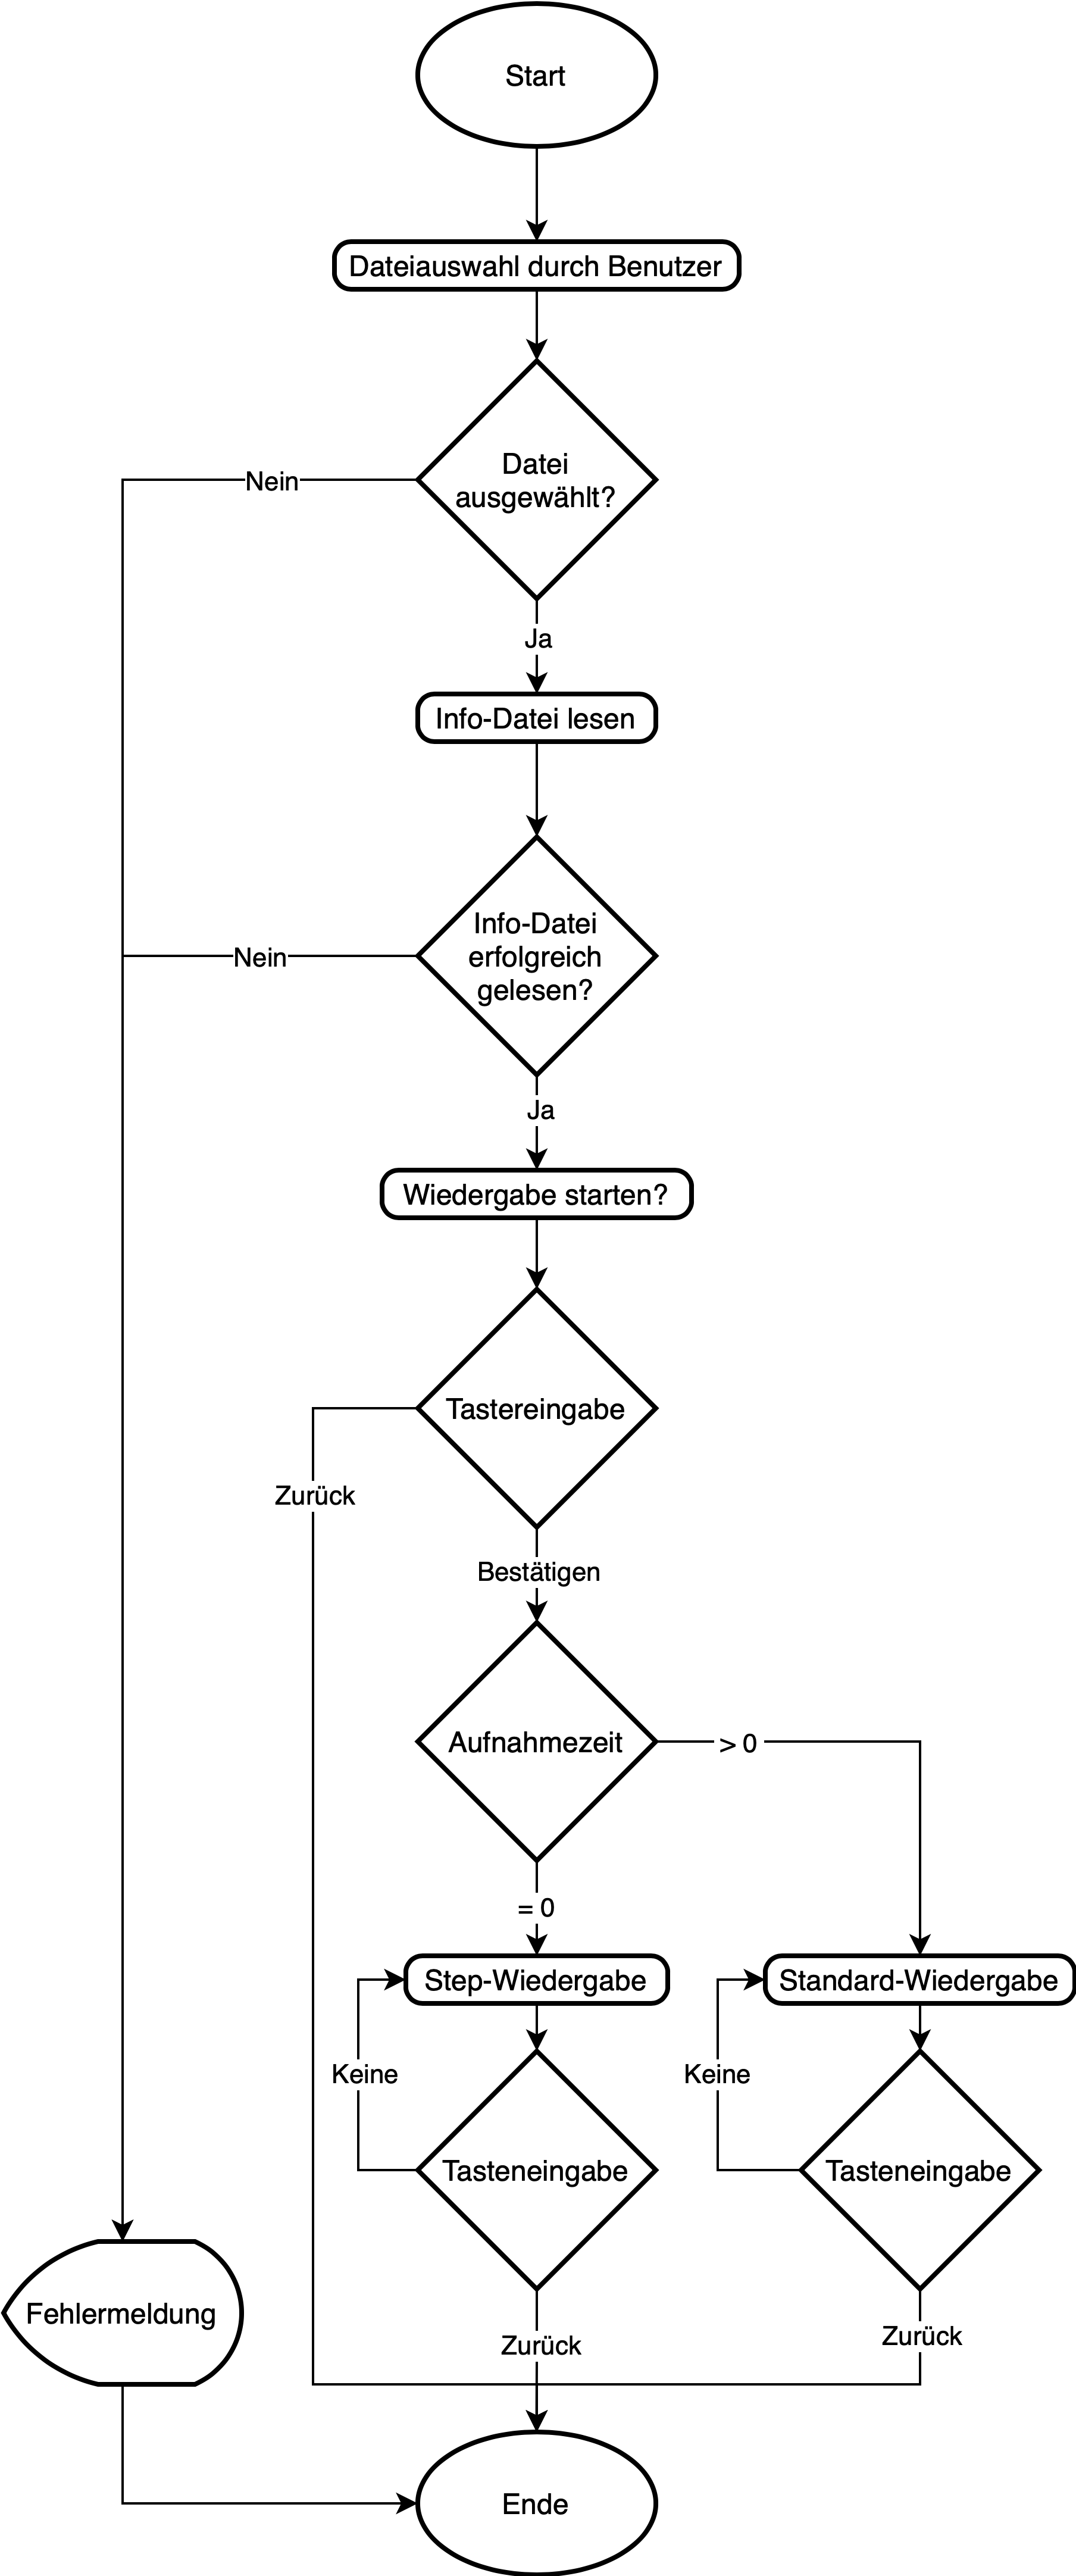
\includegraphics[height=.769\textheight]{Wiedergabefunktion}
	\end{center}
\end{figure}
\newpage
\subsection{Standard Wiedergabe}
\label{fluss:playconti}
\begin{figure}[h]
	\begin{center}
		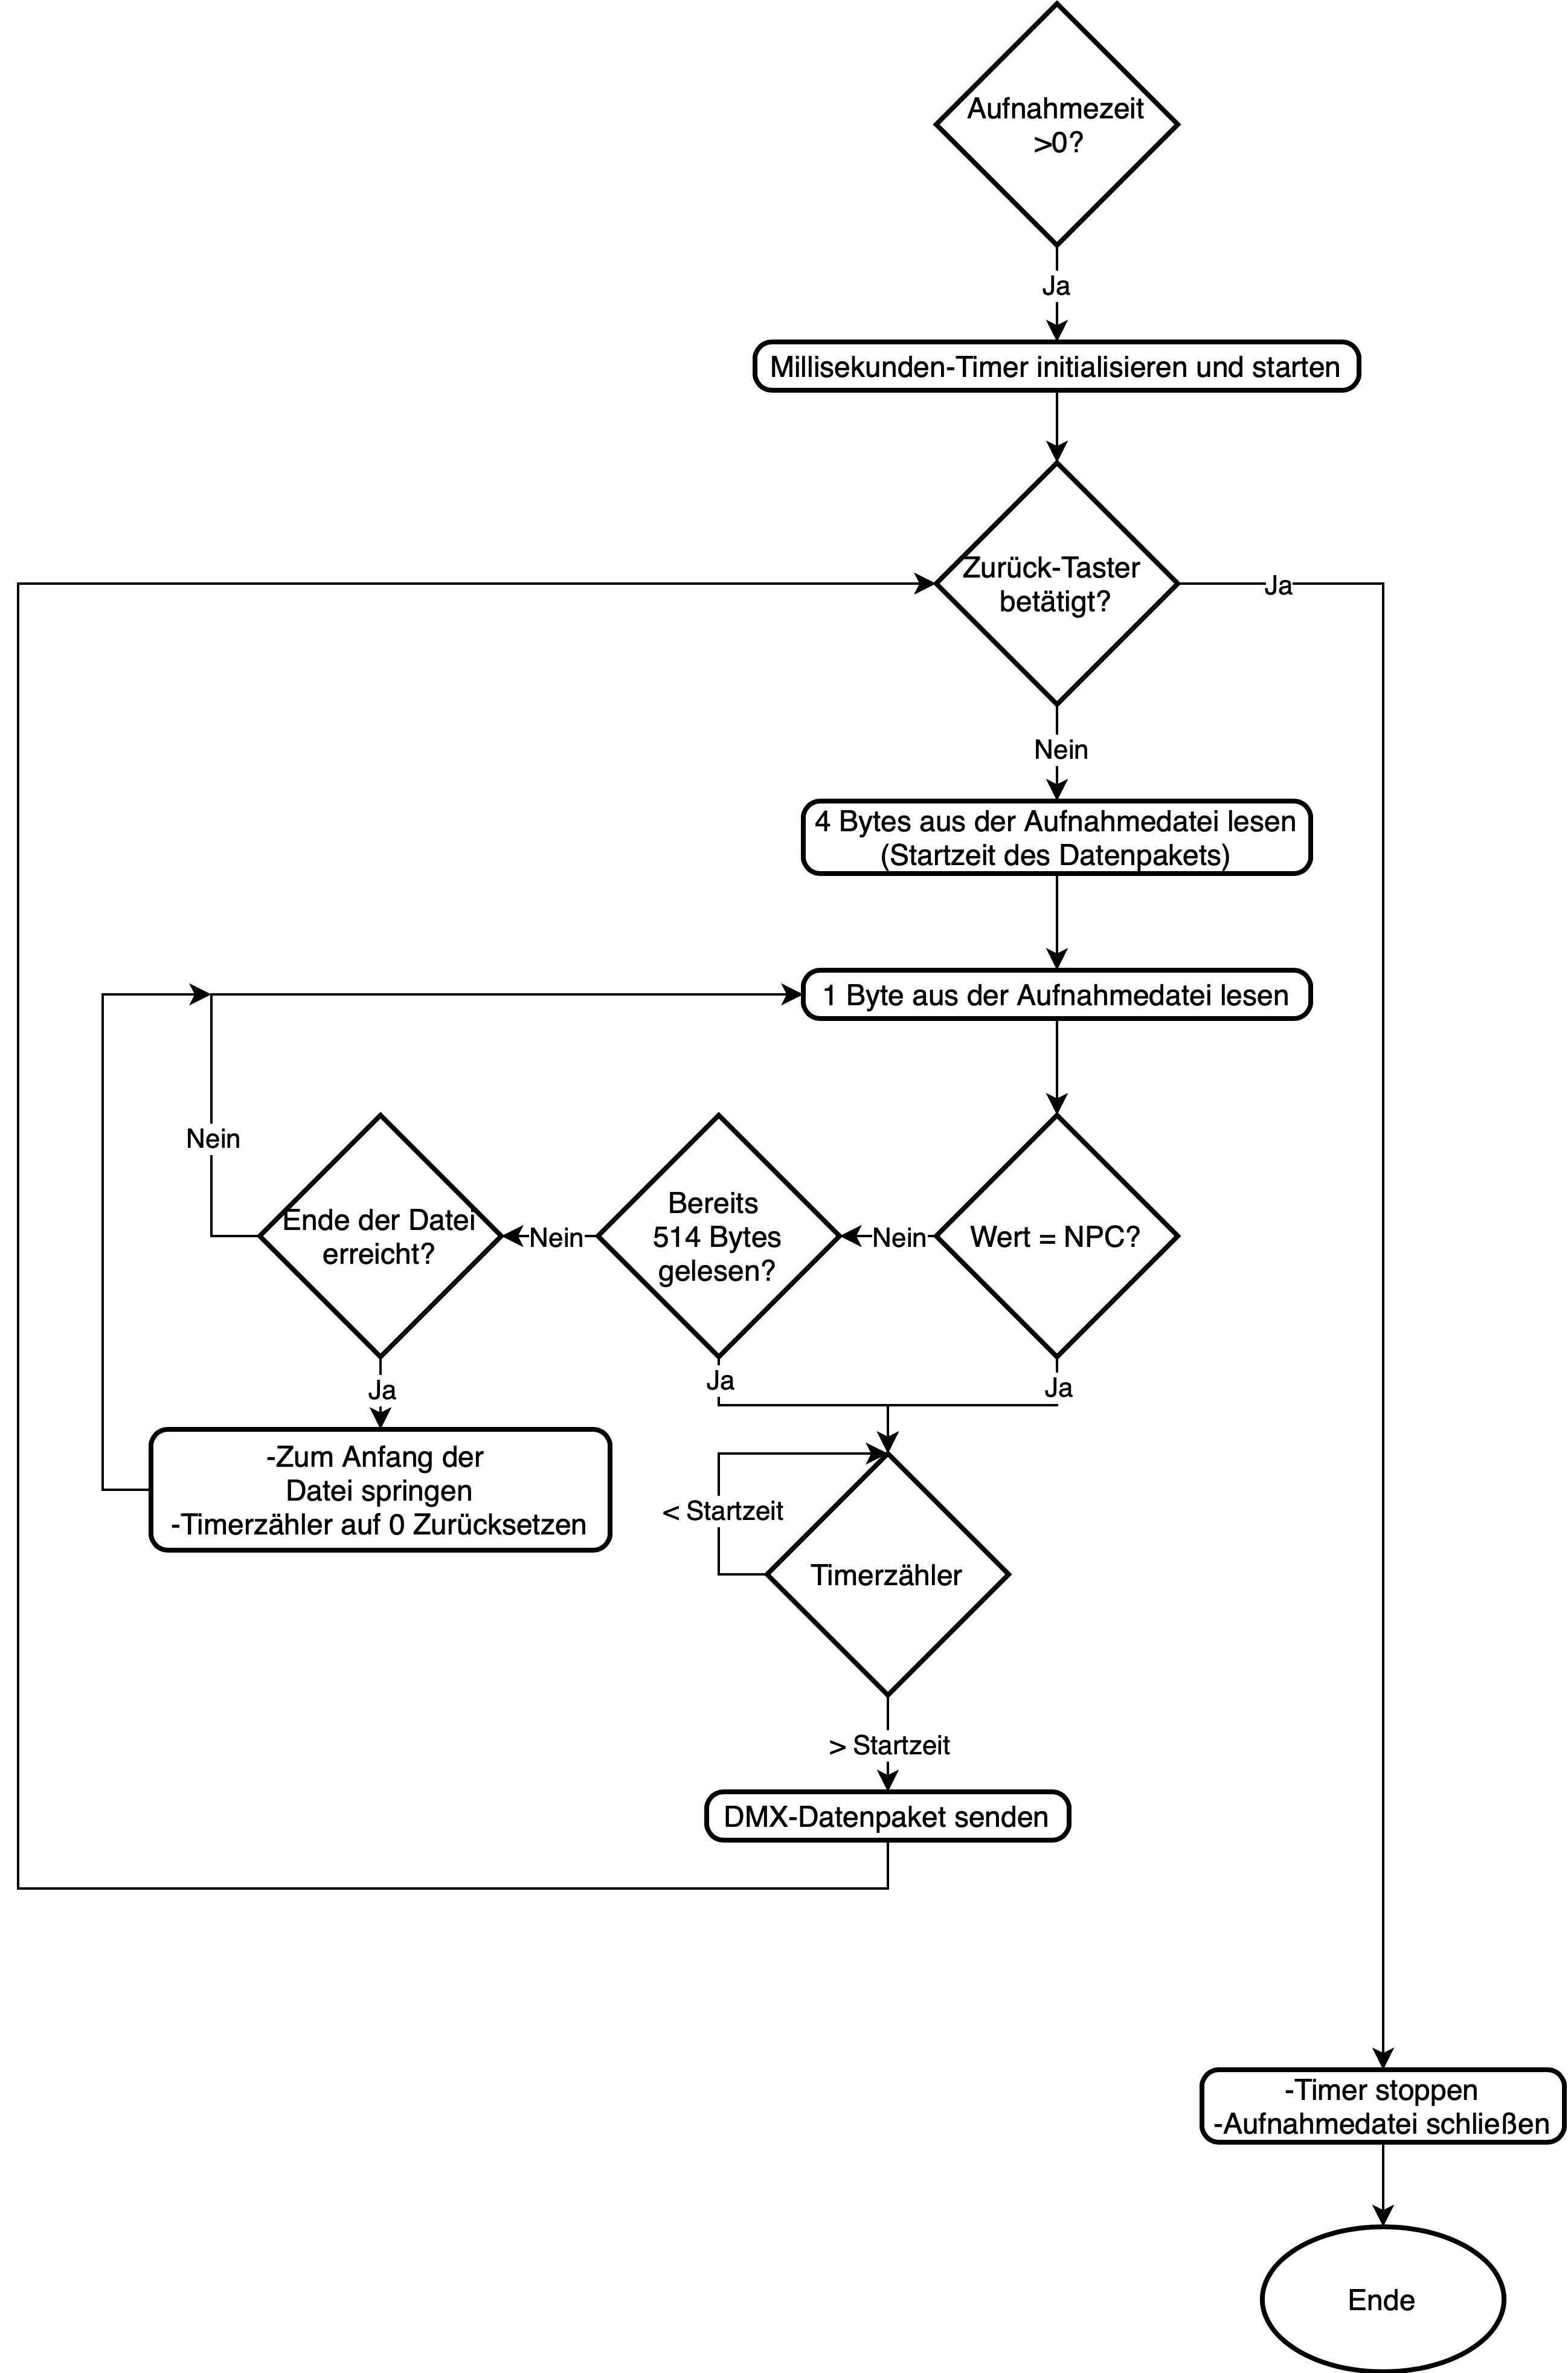
\includegraphics[height=.76\textheight]{Wiedergabe_kontinuierlich}
	\end{center}
\end{figure}
\newpage
\section{Inhalt CD-ROM}
\label{CD-Anhang}
\begin{figure}[h]
	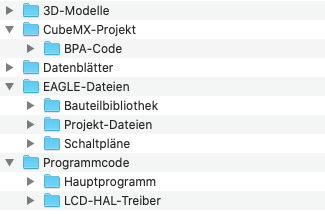
\includegraphics[scale=.7]{CD-Inhalt}
\end{figure}